\textbf{How to Structure your Submission}
\\
All submission are to take the form of a single zip file.  The zip file must maintain the folder structure as generated by 3DS Max or Unity.   The images below, figure \ref{fig:3dsstructure} and figure \ref{fig:unity} give an indication of the folder structure that you should zip and submit.

\begin{figure}[h]
	\centering
	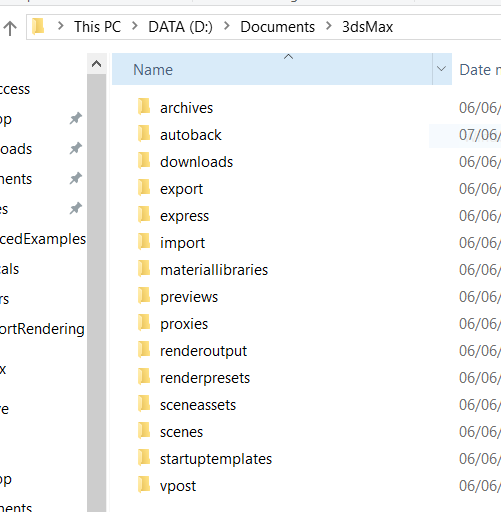
\includegraphics[width=0.5\linewidth]{img/3dsStructure.jpg}
	\caption{3D Studio Max Project Folder Structure}
	\label{fig:3dsstructure}
\end{figure}
\begin{figure}[h]
	\centering
	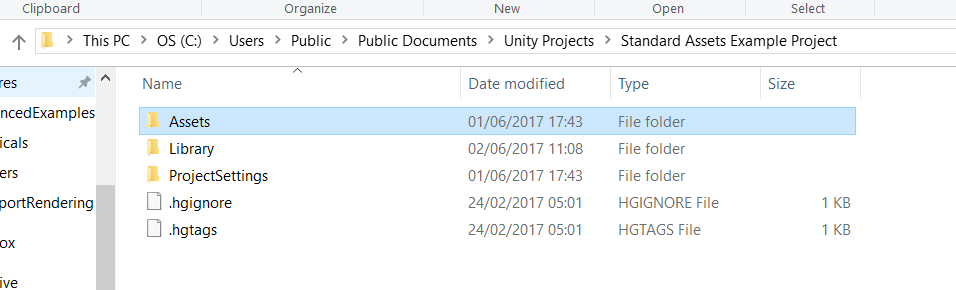
\includegraphics[width=0.9\linewidth]{img/Unity.jpg}
	\caption{Unity Game Engine File Structure}
	\label{fig:unity}
\end{figure}

All assets used during the course of the assignment are to be submitted.  All assets used and created should be placed within the appropriate folder.  To clarify, all 3ds Scene files should be placed within the 'scenes' folder; and all renders should be placed within the 'renderoutput' folder.
\\
\\
Please note that it is not appropriate to submit a single \textit{.max} file, single \textit{.jpg} file, or a single \textit{.unity} file.  